\documentclass[border=5pt]{standalone}

\usepackage{pgfplots}
\pgfplotsset{width=7cm,compat=1.5}

\begin{document}

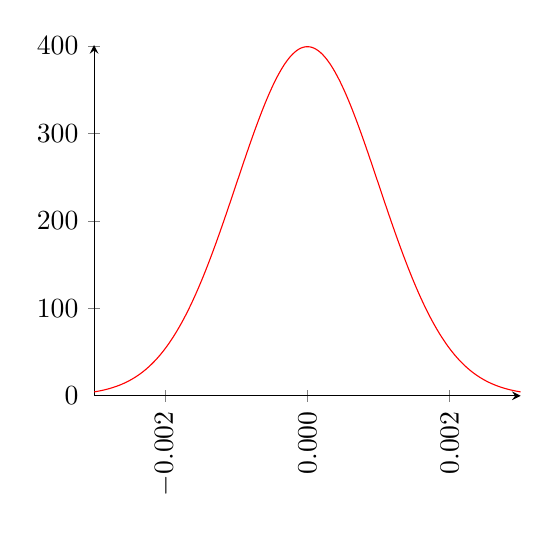
\begin{tikzpicture}
\begin{axis}[
  axis lines=left,
  scaled ticks=false,
  xticklabel style={
    rotate=90,
%    anchor=east,
    /pgf/number format/precision=3,
    /pgf/number format/fixed,
    /pgf/number format/fixed zerofill,
  },
  ymin=0,
  ymax=401,
]
  % define various constants
  \newcommand\MU{0}
  \newcommand\SIGMA{1e-3}

  \addplot[
    red,
    domain=-3*\SIGMA:3*\SIGMA,
    samples=201
  ]
  { exp(-0.5*(x-\MU)^2/\SIGMA^2)/(\SIGMA*sqrt(2*pi)) };

\end{axis}
\end{tikzpicture}

\end{document}
